\documentclass{article}
    \usepackage{ctex}
    \usepackage{graphicx}
    \usepackage{mathtools}
    \title{对Word Embedding的理解}
    \author{Yuchen Zhong}
    \date{}
    \begin{document}
        \maketitle
        \section{前言}
        词嵌入($Word Embedding$)是指将词汇映射成一个向量,这个向量称为词向量。
        引入词嵌入的目的,是为了方便计算机来处理文本。
        
        最容易想到的办法自然是哈希($hash$)。比如著名的$murmurhash$可以将任意长度的字符串
        以O(1)的复杂度直接转换成一个64位的整数。在词袋模型($BOW$)中,需要建立文档
        的词汇表并统计各个词的出现次数,存储的方式一般就是采用哈希的映射方法,然后可以利
        用$TF-IDF$,进行文章检索。

        虽然通过哈希,我们有了每个词对应的词向量,但是这个词向量显然不能反应词与词
        之间的相关度。因为哈希的算法只是一种纯粹的映射,并没有夹杂语义($semantic$)的因素。
        所以需要寻找新的词嵌入方法。

        其实甚至可以联想到$huffman$编码和$unicode$编码,不过和哈希方法一样,都只是编码方法罢了。

        另外,有人根据词袋模型,倒是给出了这样的一个方法:根据语料库,建立
        一个词汇表($Vocabulary$),给每一个词建立一个向量,长度是词汇表单词总数,
        向量的该单词在词汇表出现的位置的地方为1,向量其余全为0。这样映射方法
        称为独热码($one-hot$),每一个词向量都只有一个1。这种办法和上面说过的哈希一样,都缺乏
        语义的考虑,无法反应词与词之间的相关度。

        其实上述算法都只利用语料库了皮毛。只看到了词汇,但是没有看到上下文。
        看到这里,大概就能明确所要建立模型的目标了:不仅仅要对词进行向量化的
        表示,还要使得向量之间尽可能多地蕴含语义和语法的信息。
        下面介绍的
        $word2vec$模型才真正利用了语料库。

        \section{word2vec}
        简单地说,$word2vec$模型是利用具有隐藏层的神经网络训练得到词向量的。
        它的核心思想一样很朴素,只不过是我们日常生活中的用上下文来推断一个词的词义而已。

        神经网络需要输入和输出。对$word2vec$模型来讲,输入层和输出层的都是语料库的词汇表;
        采用one-hot的方式输入。
        另外,作为输入和输出的训练集的确有些新奇:对于每个句子,选取一个中心词$y$,
        其他上下文构成$x$;如果把上下文$x$的$one-hot$向量当做输入,而把中心词$y$看做
        输出,那么就称为$CBOW$模型;反之,对调输入输出,则称为$Skip-gram$模型。

        先从最简单的CBOW模型入手,也就是只有一个$contex$。
        如图所示:
        \begin{center}
            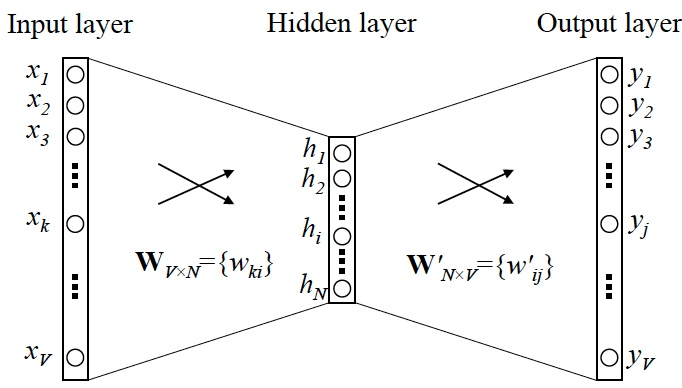
\includegraphics[scale=0.4]{1.jpg}
        \end{center}
        
        因为在输入向量$\mathbf{x}=\{x_1,x_2...,x_V\}$中,有且只有一个$x_k$为1,
        所以易知,
        \begin{equation}
            \mathbf{h} = \mathbf{W^{T}x} = \mathbf{W_{(k,·)}^{T}} := \mathbf{v}_{k}^\mathbf{T}
        \end{equation}
        也就是说,隐藏层的向量值其实就是权值矩阵的第$k$行的向量值,

        隐藏层采用线性的激活函数(关于这一点我认为是对模型的简化),可以认为隐层不做
        任何处理直接输出。继续推下一层,易知输出层的输入值满足如下关系:
        \begin{equation}
            u_j = \mathbf{v}'^{T}_{w_j}\mathbf{h}
        \end{equation}
        最后输出采用softmax计算概率,如下所示:
        \begin{equation}
            y_j = \frac{exp(u_j)}{\Sigma_{j'=1}^{V}exp(u_j')}
        \end{equation}
        这个概率代表什么呢?很明显,是已知出现输入的
        $contex$的情况下,词汇表中每个词出现的概率是多大用条件概率来表示即为:
        \[ p(w_j|w_{contex}) := y_j\]
        当然我们拥有
        语料库,是已知标准答案的(也就是真正出现的中心词)。
        不妨假设标准答案所在词汇表的位置是$j^*$。
        所以我们的目标,就是极大化标准答案的出现概率。
        \begin{equation}
            \begin{split}
                max\quad p(w_{j^*}|w_{contex}) &= max\quad y_{j^*} \\
                                         &= max\quad log(y_j^*) \\
                                         &= max\quad u_{j^*} - log \Sigma_{j'=1}^{V}exp(u_j')
            \end{split}
        \end{equation}
        令
        \begin{equation}
            E := -log p(w_{j^*}|w_{contex}) 
        \end{equation}
        为损失函数,我们目标转为minimize E。

        后面就是传统的反向传播(backpropagation)过程,不再详细推导。最终神经
        网络会收敛,从input层到hidden层的权重就是我们要的词向量!

        上面介绍的是最简单的一个单词做contex的情况,如果多个单词作contex呢?
        只需要把(1)式变为:
        \begin{equation}
            \mathbf{h} = \mathbf{W^{T}}(x_1+x_2+...+x_C)
        \end{equation}
        即可。

        这种方法的确非常巧妙。更让人意外的,是word2vec还具有很好的性质。

        最著名的就是类比性(analogy),如 v(国王) - v(王后) = v(男人) - v(女人)。
        但非常可惜,这个只是实验发现的,到目前并没有很好地解释。


        \section{GloVe}
            待更……






        

        

    \end{document}